\documentclass{standalone}
\usepackage{tikz}
\usetikzlibrary{patterns, positioning}


\begin{document}
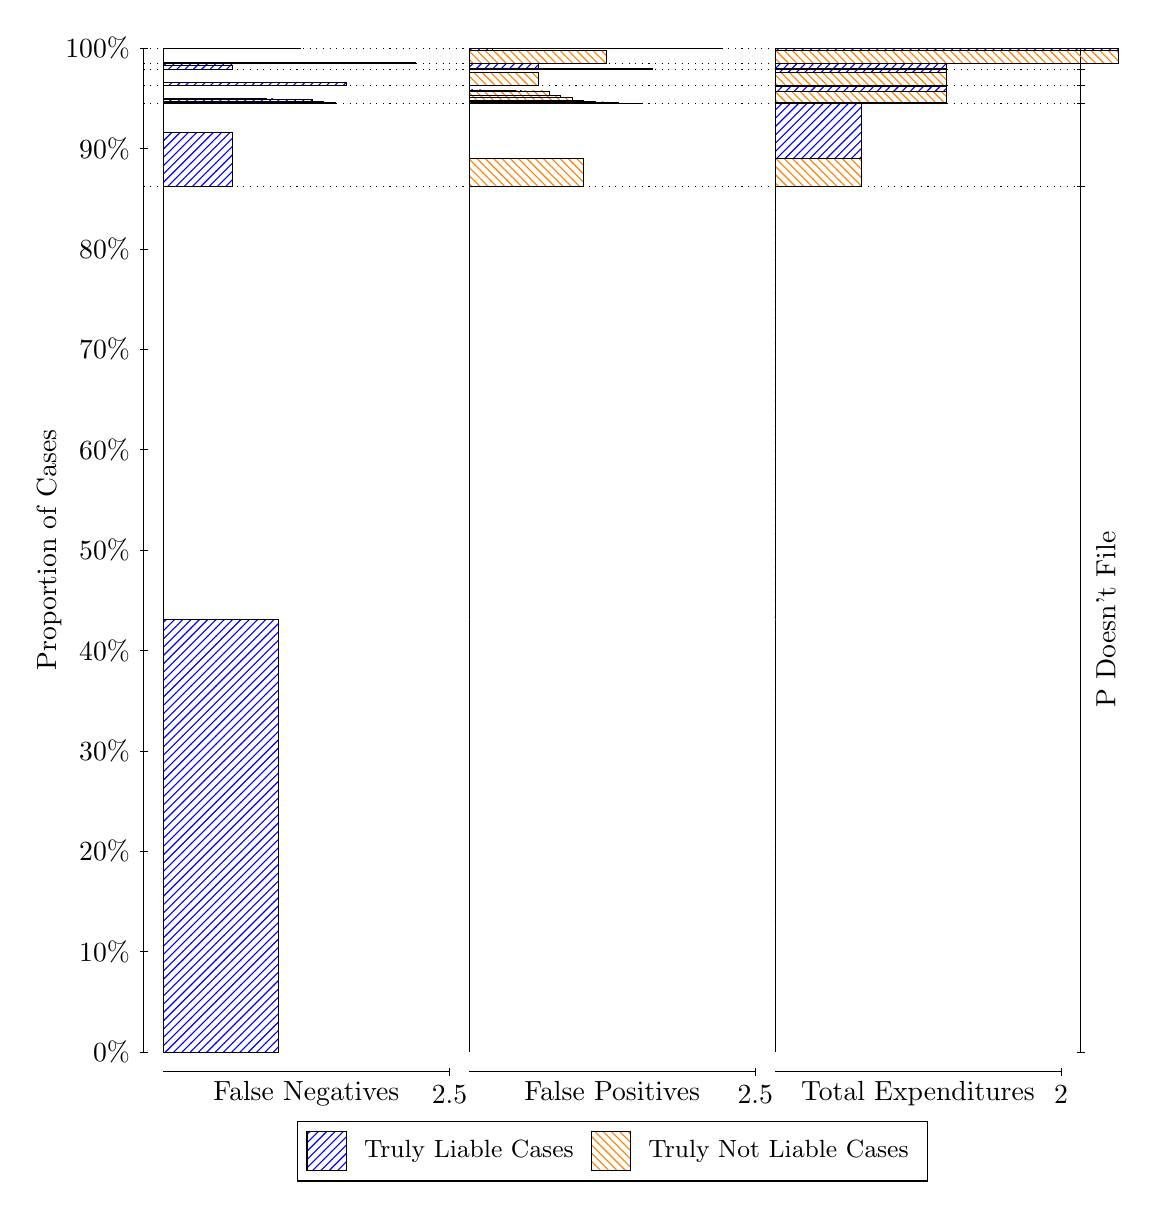
\begin{tikzpicture}
\draw[black, very thin] (1.5,1.75) -- (1.5,14.5);
\node[rotate=90, text=black, anchor=center] at (0.3, 8.125) {Proportion of Cases};
\draw[black, very thin] (1.45,1.75) -- (1.55,1.75);
\node[text=black, anchor=east] at (1.45, 1.75) {0\%};
\draw[black, very thin] (1.45,3.025) -- (1.55,3.025);
\node[text=black, anchor=east] at (1.45, 3.025) {10\%};
\draw[black, very thin] (1.45,4.3) -- (1.55,4.3);
\node[text=black, anchor=east] at (1.45, 4.3) {20\%};
\draw[black, very thin] (1.45,5.575) -- (1.55,5.575);
\node[text=black, anchor=east] at (1.45, 5.575) {30\%};
\draw[black, very thin] (1.45,6.85) -- (1.55,6.85);
\node[text=black, anchor=east] at (1.45, 6.85) {40\%};
\draw[black, very thin] (1.45,8.125) -- (1.55,8.125);
\node[text=black, anchor=east] at (1.45, 8.125) {50\%};
\draw[black, very thin] (1.45,9.4) -- (1.55,9.4);
\node[text=black, anchor=east] at (1.45, 9.4) {60\%};
\draw[black, very thin] (1.45,10.675) -- (1.55,10.675);
\node[text=black, anchor=east] at (1.45, 10.675) {70\%};
\draw[black, very thin] (1.45,11.95) -- (1.55,11.95);
\node[text=black, anchor=east] at (1.45, 11.95) {80\%};
\draw[black, very thin] (1.45,13.225) -- (1.55,13.225);
\node[text=black, anchor=east] at (1.45, 13.225) {90\%};
\draw[black, very thin] (1.45,14.5) -- (1.55,14.5);
\node[text=black, anchor=east] at (1.45, 14.5) {100\%};

\draw[black, very thin] (13.4,1.75) -- (13.4,14.5);
\draw[black, very thin] (13.35,1.75) -- (13.45,1.75);
\node[anchor=west] at (13.35, 1.75) {};
\draw[black, very thin] (13.35,12.738) -- (13.45,12.738);
\node[anchor=west] at (13.35, 12.738) {};
\draw[black, very thin] (13.35,13.792) -- (13.45,13.792);
\node[anchor=west] at (13.35, 13.792) {};
\draw[black, very thin] (13.35,14.024) -- (13.45,14.024);
\node[anchor=west] at (13.35, 14.024) {};
\draw[black, very thin] (13.35,14.224) -- (13.45,14.224);
\node[anchor=west] at (13.35, 14.224) {};
\draw[black, very thin] (13.35,14.3) -- (13.45,14.3);
\node[anchor=west] at (13.35, 14.3) {};
\draw[black, very thin] (13.35,14.491) -- (13.45,14.491);
\node[anchor=west] at (13.35, 14.491) {};
\draw[black, very thin] (13.35,14.5) -- (13.45,14.5);
\node[anchor=west] at (13.35, 14.5) {};

\draw[black, very thin, pattern color=blue, pattern=north east lines] (1.75,1.75) rectangle (3.2033,7.244);
\draw[black, very thin, pattern color=orange, pattern=north west lines] (1.75,7.244) rectangle (1.75,12.738);
\draw[black, very thin, pattern color=blue, pattern=north east lines] (1.75,12.738) rectangle (2.622,13.427);
\draw[black, very thin, pattern color=orange, pattern=north west lines] (1.75,13.427) rectangle (1.75,13.792);
\draw[black, very thin, pattern color=blue, pattern=north east lines] (1.75,13.792) rectangle (3.93,13.806);
\draw[black, very thin, pattern color=blue, pattern=north east lines] (1.75,13.806) rectangle (3.7847,13.824);
\draw[black, very thin, pattern color=blue, pattern=north east lines] (1.75,13.824) rectangle (3.6393,13.844);
\draw[black, very thin, pattern color=blue, pattern=north east lines] (1.75,13.844) rectangle (3.494,13.847);
\draw[black, very thin, pattern color=blue, pattern=north east lines] (1.75,13.847) rectangle (3.3487,13.851);
\draw[black, very thin, pattern color=blue, pattern=north east lines] (1.75,13.851) rectangle (3.2033,13.854);
\draw[black, very thin, pattern color=blue, pattern=north east lines] (1.75,13.854) rectangle (3.058,13.857);
\draw[black, very thin, pattern color=blue, pattern=north east lines] (1.75,13.857) rectangle (2.9127,13.858);
\draw[black, very thin, pattern color=blue, pattern=north east lines] (1.75,13.858) rectangle (2.7673,13.86);
\draw[black, very thin, pattern color=orange, pattern=north west lines] (1.75,13.86) rectangle (1.75,14.024);
\draw[black, very thin, pattern color=blue, pattern=north east lines] (1.75,14.024) rectangle (4.0753,14.062);
\draw[black, very thin, pattern color=orange, pattern=north west lines] (1.75,14.062) rectangle (1.75,14.224);
\draw[black, very thin, pattern color=blue, pattern=north east lines] (1.75,14.224) rectangle (2.622,14.286);
\draw[black, very thin, pattern color=orange, pattern=north west lines] (1.75,14.286) rectangle (1.75,14.3);
\draw[black, very thin, pattern color=blue, pattern=north east lines] (1.75,14.3) rectangle (4.9473,14.319);
\draw[black, very thin, pattern color=orange, pattern=north west lines] (1.75,14.319) rectangle (1.75,14.491);
\draw[black, very thin, pattern color=blue, pattern=north east lines] (1.75,14.491) rectangle (3.494,14.496);
\draw[black, very thin, pattern color=orange, pattern=north west lines] (1.75,14.496) rectangle (1.75,14.5);
\draw[black, very thin, pattern color=orange, pattern=north west lines] (5.6333,1.75) rectangle (5.6333,7.244);
\draw[black, very thin, pattern color=blue, pattern=north east lines] (5.6333,7.244) rectangle (5.6333,12.738);
\draw[black, very thin, pattern color=orange, pattern=north west lines] (5.6333,12.738) rectangle (7.0867,13.103);
\draw[black, very thin, pattern color=blue, pattern=north east lines] (5.6333,13.103) rectangle (5.6333,13.792);
\draw[black, very thin, pattern color=orange, pattern=north west lines] (5.6333,13.792) rectangle (7.8133,13.795);
\draw[black, very thin, pattern color=orange, pattern=north west lines] (5.6333,13.795) rectangle (7.668,13.799);
\draw[black, very thin, pattern color=orange, pattern=north west lines] (5.6333,13.799) rectangle (7.5227,13.807);
\draw[black, very thin, pattern color=orange, pattern=north west lines] (5.6333,13.807) rectangle (7.3773,13.815);
\draw[black, very thin, pattern color=orange, pattern=north west lines] (5.6333,13.815) rectangle (7.232,13.827);
\draw[black, very thin, pattern color=orange, pattern=north west lines] (5.6333,13.827) rectangle (7.0867,13.834);
\draw[black, very thin, pattern color=orange, pattern=north west lines] (5.6333,13.834) rectangle (6.9413,13.87);
\draw[black, very thin, pattern color=orange, pattern=north west lines] (5.6333,13.87) rectangle (6.796,13.899);
\draw[black, very thin, pattern color=orange, pattern=north west lines] (5.6333,13.899) rectangle (6.6507,13.956);
\draw[black, very thin, pattern color=blue, pattern=north east lines] (5.6333,13.956) rectangle (6.36,13.957);
\draw[black, very thin, pattern color=blue, pattern=north east lines] (5.6333,13.957) rectangle (6.2147,13.959);
\draw[black, very thin, pattern color=blue, pattern=north east lines] (5.6333,13.959) rectangle (6.0693,13.962);
\draw[black, very thin, pattern color=blue, pattern=north east lines] (5.6333,13.962) rectangle (5.924,13.965);
\draw[black, very thin, pattern color=blue, pattern=north east lines] (5.6333,13.965) rectangle (5.7787,13.969);
\draw[black, very thin, pattern color=blue, pattern=north east lines] (5.6333,13.969) rectangle (5.6333,14.024);
\draw[black, very thin, pattern color=orange, pattern=north west lines] (5.6333,14.024) rectangle (6.5053,14.186);
\draw[black, very thin, pattern color=blue, pattern=north east lines] (5.6333,14.186) rectangle (5.6333,14.224);
\draw[black, very thin, pattern color=orange, pattern=north west lines] (5.6333,14.224) rectangle (7.9587,14.238);
\draw[black, very thin, pattern color=blue, pattern=north east lines] (5.6333,14.238) rectangle (6.5053,14.3);
\draw[black, very thin, pattern color=orange, pattern=north west lines] (5.6333,14.3) rectangle (7.3773,14.471);
\draw[black, very thin, pattern color=blue, pattern=north east lines] (5.6333,14.471) rectangle (5.924,14.491);
\draw[black, very thin, pattern color=orange, pattern=north west lines] (5.6333,14.491) rectangle (8.8307,14.495);
\draw[black, very thin, pattern color=blue, pattern=north east lines] (5.6333,14.495) rectangle (7.3773,14.5);
\draw[black, very thin, pattern color=orange, pattern=north west lines] (9.5167,1.75) rectangle (9.5167,7.244);
\draw[black, very thin, pattern color=blue, pattern=north east lines] (9.5167,7.244) rectangle (9.5167,12.738);
\draw[black, very thin, pattern color=orange, pattern=north west lines] (9.5167,12.738) rectangle (10.607,13.103);
\draw[black, very thin, pattern color=blue, pattern=north east lines] (9.5167,13.103) rectangle (10.607,13.792);
\draw[black, very thin, pattern color=orange, pattern=north west lines] (9.5167,13.792) rectangle (11.697,13.803);
\draw[black, very thin, pattern color=blue, pattern=north east lines] (9.5167,13.803) rectangle (11.697,13.808);
\draw[black, very thin, pattern color=orange, pattern=north west lines] (9.5167,13.808) rectangle (11.697,13.948);
\draw[black, very thin, pattern color=blue, pattern=north east lines] (9.5167,13.948) rectangle (11.697,14.008);
\draw[black, very thin, pattern color=orange, pattern=north west lines] (9.5167,14.008) rectangle (11.697,14.019);
\draw[black, very thin, pattern color=blue, pattern=north east lines] (9.5167,14.019) rectangle (11.697,14.024);
\draw[black, very thin, pattern color=orange, pattern=north west lines] (9.5167,14.024) rectangle (11.697,14.186);
\draw[black, very thin, pattern color=blue, pattern=north east lines] (9.5167,14.186) rectangle (11.697,14.224);
\draw[black, very thin, pattern color=orange, pattern=north west lines] (9.5167,14.224) rectangle (11.697,14.238);
\draw[black, very thin, pattern color=blue, pattern=north east lines] (9.5167,14.238) rectangle (11.697,14.3);
\draw[black, very thin, pattern color=orange, pattern=north west lines] (9.5167,14.3) rectangle (13.877,14.471);
\draw[black, very thin, pattern color=blue, pattern=north east lines] (9.5167,14.471) rectangle (13.877,14.491);
\draw[black, very thin, pattern color=orange, pattern=north west lines] (9.5167,14.491) rectangle (13.877,14.495);
\draw[black, very thin, pattern color=blue, pattern=north east lines] (9.5167,14.495) rectangle (13.877,14.5);
\draw[black, dotted] (1.5,12.738) -- (13.4,12.738);
\draw[black, dotted] (1.5,13.792) -- (13.4,13.792);
\draw[black, dotted] (1.5,14.024) -- (13.4,14.024);
\draw[black, dotted] (1.5,14.224) -- (13.4,14.224);
\draw[black, dotted] (1.5,14.3) -- (13.4,14.3);
\draw[black, dotted] (1.5,14.491) -- (13.4,14.491);
\draw[black, very thin] (1.75,1.5) -- (5.3833,1.5);
\node[text=black, anchor=north] at (3.5667, 1.5) {False Negatives};
\draw[black, very thin] (5.3833,1.45) -- (5.3833,1.55);
\node[text=black, anchor=north] at (5.3833, 1.45) {2.5};

\draw[black, very thin] (5.6333,1.5) -- (9.2667,1.5);
\node[text=black, anchor=north] at (7.45, 1.5) {False Positives};
\draw[black, very thin] (9.2667,1.45) -- (9.2667,1.55);
\node[text=black, anchor=north] at (9.2667, 1.45) {2.5};

\draw[black, very thin] (9.5167,1.5) -- (13.15,1.5);
\node[text=black, anchor=north] at (11.333, 1.5) {Total Expenditures};
\draw[black, very thin] (13.15,1.45) -- (13.15,1.55);
\node[text=black, anchor=north] at (13.15, 1.45) {2};

\node[text=black, centered, rotate=90] at (13.72, 7.244) {P Doesn't File};







\draw (7.449999999999999,1.5) node[draw=none] (baseCoordinate) {};
\begin{scope}[align=center]
        \matrix[scale=0.5, draw=black, below=0.5cm of baseCoordinate, nodes={draw}, column sep=0.1cm]{
            \node[rectangle, draw, minimum width=0.5cm, minimum height=0.5cm, pattern color=blue, pattern=north east lines] {}; &
            \node[draw=none, font=\small, text=black] (B) {Truly Liable Cases}; &
            \node[rectangle, draw, minimum width=0.5cm, minimum height=0.5cm, pattern color=orange, pattern=north west lines] {}; &
            \node[draw=none, font=\small, text=black] (B) {Truly Not Liable Cases}; \\
            };
\end{scope}

\end{tikzpicture}
\end{document}